



\documentclass{article}
\usepackage{amsmath, amsthm}
\usepackage{amssymb}
\usepackage{mathtools}
\usepackage[all,cmtip]{xy}
\usepackage{color}


\setcounter{tocdepth}{4}

\renewenvironment{proof}{ {\bfseries Proof:}}{\qed}

\newtheoremstyle{mytheorem}%                % Name
{}%                                     % Space above
{}%                                     % Space below
{\itshape}%                                     % Body font
{0pt}%\parindent}%                                     % Indent amount
{\bfseries}%                            % Theorem head font
{.}%                                    % Punctuation after theorem head
{ }%                                    % Space after theorem head, ' ', or \newline
{}%                                     % Theorem head spec (can be left empty, meaning `normal')

\theoremstyle{mytheorem}
\newtheorem{thm}{Theorem}[section]
\newtheorem{proposition}[thm]{Proposition}
\newtheorem{lemma}[thm]{Lemma}
\newtheorem{corollary}[thm]{Corollary}


\newtheoremstyle{mydefinition}%                % Name
{}%                                     % Space above
{}%                                     % Space below
{}%                                     % Body font
{0pt}%\parindent}%                                     % Indent amount
{\bfseries}%                            % Theorem head font
{.}%                                    % Punctuation after theorem head
{ }%                                    % Space after theorem head, ' ', or \newline
{}%                                     % Theorem head spec (can be left empty, meaning `normal')

\theoremstyle{mydefinition}
\newtheorem{definition}[thm]{Definition}
\newtheorem{example}[thm]{Example}
\newtheorem{exercise}[thm]{Exercise}
\newtheorem{remark}[thm]{Remark}
%\newtheorem{ques}[thm]{Q.}
\newtheorem*{ques}{Question}
%\newtheorem{ans}[thm]{Ans.}
\newtheorem*{ans}{Ans}



\numberwithin{equation}{section}

%Real numbers, complex numbers, etc.
\newcommand{\R}{\mathbb{R}}
\newcommand{\C}{\mathbb{C}}
\newcommand{\Z}{\mathbb{Z}}
\newcommand{\Q}{\mathbb{Q}}
\renewcommand{\P}{\mathbb{P}}

%How does latex not have these?
\DeclareMathOperator{\Ad}{Ad}
\DeclareMathOperator{\ad}{ad}
\DeclareMathOperator{\tr}{tr}
\DeclareMathOperator{\Tr}{Tr}
\DeclareMathOperator{\Hom}{Hom}
\DeclareMathOperator{\Spec}{Spec}
\DeclareMathOperator{\im}{im}
\DeclareMathOperator{\rank}{rank}
\DeclareMathOperator{\Exists}{\exists}
\DeclareMathOperator{\Forall}{\forall}

\DeclareMathOperator*{\colim}{colim}
\DeclareMathOperator*{\holim}{holim}
\DeclareMathOperator*{\hocolim}{hocolim}


%fractions and inner product
\newcommand{\pr}[2][\:]{\frac{\partial #1}{\partial #2}}
\newcommand{\innerp}[2]{\langle #1, #2 \rangle}

\newcommand*\conj[1]{\overline{#1}}
\newcommand*\norm[1]{\lVert #1 \rVert}

\renewcommand{\figurename}{Fig.}
\usepackage{float}
\usepackage{wrapfig}

\usepackage{enumitem}
\setlist[enumerate]{itemsep=0mm}
\usepackage{geometry}
\geometry{
	a4paper,
	total={170mm,257mm},
	left=20mm,
	top=20mm
}


\usepackage{fancyhdr}
\pagestyle{fancy}
\lhead{\scshape Apurva Nakade}
%\rhead{\scshape Mathcamp 2017}
\renewcommand*{\thepage}{\small\arabic{page}}


\renewcommand{\thefootnote}{\fnsymbol{footnote}}

\begin{document}
\title{Euler Characteristic of the Sphere}
\author{Apurva Nakade}
\maketitle

A topological invariant assigns to a topological space, in our case a surface, an algebraic object such as a number, a polynomial or a vector space. If two surfaces have different topological invariants then they must be topologically inequivalent. (However the converse is not always true in that two inequivalent surfaces can have the same topological invariants.) The simplest non-trivial topological invariant is the Euler characteristic. The Euler characteristic assigns to each surface an integer and can be thought of as a way of quantifying shapes.

Euler characteristic for surfaces is computed using graphs. We begin with the simplest surface, the sphere $ S ^ 2 $.

\begin{example}
	For a polyhedron $P$ let $v,e,f$ denote the number of vertices, edges and faces respectively. When $P$ is a tetrahedron $v = 4, e=6, f=4$ and hence $v-e+f = 2$. When $P$ is a cube $v = 8, e=12, f=6$ and hence $v-e+f = 2$.
\end{example}

What does the cube and the tetrahedron have in common? They can all be continuously deformed to the 2 dimensional sphere $ S^2 $.



\section{Planar graphs}
We'll start by computing the Euler characteristic of a planar graph. For us a graph $ G $ is a pair of finite sets $(V,E) $ where the vertices, $ V $, are distinct points in the standard plane $ \R ^2 $ and the edges, $ E $, are segments connecting two vertices. We say that a graph is \textbf{connected} if each vertex is connected to every other vertex via a sequence of edges. We say that a graph is \textbf{planar} if no two edges intersect in a point outside the set of vertices.


A planar graph divides the plane $ \R ^ 2 $ into \textbf{faces}. Denote the set of faces by $ F $.\footnote{We won't include the unbounded face in $F$, for us all the faces are (possibly non-convex) polygons.} (It is possible for the set $ F $ to be empty.) The \textbf{Euler characteristic} of a planar graph $ G $ is defined to be
\begin{align*}
	\chi (G):= |V| - |E| + |F|
\end{align*}
where $ |S| $ denotes the size of the set $ S $.

\begin{thm}\label{thm:euler_characteristic_of_graphs}
	The Euler characteristic of a connected planar graph is 1.
\end{thm}

Exercise \ref{proof_of_euler's_thm} describes one proof of this theorem using induction on the number of faces. First we prove the theorem in the case when the graph has no faces.

A \emph{connected} graph $ G $ without any face, i.e. when $ F $ is an empty set  or equivalently $ |F| = 0 $, is called a \textbf{tree}. (A graph with no faces but which is not necessarily connected is called a forest!) A vertex in a tree with only one edge attached to it is called a \textbf{leaf}.

\begin{exercise}
	For a tree $ G $ what is the relationship between $ |V| $ and $ |E| $? What is $ \chi (G)$?
\end{exercise}

\begin{exercise}\label{proof_of_euler's_thm}
	The following is the proof of \eqref{thm:euler_characteristic_of_graphs}
	\begin{enumerate}
		\item For a connected planar graph $ G $ with at least 1 face, show that it is possible to delete an edge and obtain a graph $ G' $ such that $G' $ has exactly one less face than $ G $.
		\item What is the relationship between the Euler characteristic of $ G $ and $ G' $?
		\item Induct on $ |F| $ to complete the proof of Theorem \ref{thm:euler_characteristic_of_graphs}. (What is the base case for induction here?)
	\end{enumerate}
\end{exercise}

\begin{exercise}
	What is the Euler characteristic of a planar graph which is not necessarily connected?
\end{exercise}






\section{Euler characteristic of $ S ^ 2 $}

A \textbf{surface graph} on a sphere $ S ^ 2 $ is a \emph{connected planar} graph $ G = (V,E) $ such that $ V $ and $ E $ are now on $ S ^ 2 $ and all the faces are \textbf{polygons}. The tetrahedron, the cube, and the octahedron, provide examples of such surface graphs. A surface graph is called a \textbf{triangulation} if all the faces are triangles.

\begin{thm}\label{thm:euler_characteristic_of_sphere}
	The Euler characteristic of any surface graph $G$	on $ S ^ 2 $ is 2. Hence we can define the Euler characteristic of $ S^2 $ as $\chi(S^2):= \chi(G)$ and we have, $$ \chi(S ^ 2) = 2 $$
\end{thm}


\begin{exercise}
	Theorem \ref{thm:euler_characteristic_of_sphere} follows directly from Theorem \ref{thm:euler_characteristic_of_graphs} for planar graphs,
	\begin{enumerate}
		\item Explain how a surface graph on $ S ^ 2 $ gives rise to a planar graph on $ \R ^ 2 $.
		\item Draw the planar graphs for the cube, the tetrahedron and the octahedron.
		\item Show that the Euler characteristic of a graph on $ S ^ 2 $ is 2.
	\end{enumerate}
\end{exercise}

\section{Brussel Sprouts}
The game of \textbf{Brussel Sprouts} starts with 2 crosses. Each move involves joining two free ends with a curve not crossing any existing line and then putting a short stroke across the line to create two new free ends. The game ends when no such move is possible.
\begin{center}
	\begin{tabular}{c}
		{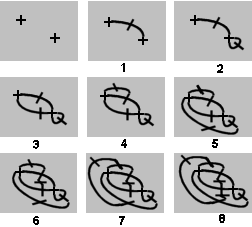
\includegraphics[width=5cm, height=5cm] {images/brussel_sprouts}} \\
		A game of Brussel Sprouts                                          \\\\
	\end{tabular}
\end{center}

\begin{exercise}
	Play a few games of Brussel Sprouts!
\end{exercise}

It turns out that every game of Brussel Sprouts always ends in the same number of steps! The following exercises describe a proof of it,

\begin{exercise}Let $G$ be the connected planar graph (vertices are the crosses) at the end of the game.
	\begin{enumerate}
		\item What happens to the number of free ends after each move? How many free ends are there in the end?
		\item Argue that at each stage of the game every face should have at least one open end on it's boundary. Further, argue that there cannot be two or more open ends on the boundary of a face at the end of the game. Hence every face of $G$ should have exactly 1 open end on it's boundary. The same is true for the \textit{unbounded face}.
		\item Conclude that $G$ has 7 faces.
	\end{enumerate}
\end{exercise}

\begin{exercise}
	Assume that the game ends in $ \mathbf{n} $ steps.
	\begin{enumerate}
		\item How many vertices and edges are added after each move? Argue that $ |E| = 2n $ and $ |V| = 2 + n $.
		\item Use Theorem \ref{thm:euler_characteristic_of_graphs} to find $ n $.
	\end{enumerate}
\end{exercise}
Can you generalize the above proof to $k$ crosses in the beginning? How about playing Brussel Sprouts on a Torus?

\iffalse\subsection{Platonic Solids}
A platonic solid is a convex polyhedron all of whose faces are regular polygons which are congruent to each other, i.e. all the edges have the same length and all the faces have the same number of sides. We'll assume that the word convex means that the platonic solid is topologically equivalent to $S^2$. We've seen 3 platonic solids earlier, the cube, the tetrahedron, and the octahedron. There are exactly two more,

\begin{center}\begin{tabular}{c c}
	%\includegraphics[width=3cm, height=3cm]{icosahedron} & %\includegraphics[width=3cm, height=3cm]{dodecahedron} \\
	icosahedron & dodecahedron \\\\
	\end{tabular}
\end{center}

We can use the Euler characteristic to prove that these 5 are the only ones possible.

Consider a platonic solid $ S $ and think of it as the graph $(V,E,F)$. Suppose all the faces of $ S $ are polygons with $ \mathbf{n} $ number of edges. Further suppose that $ \mathbf{p} $ edges of $S $ intersect at a single vertex.

\begin{exercise}
	Argue that both $ n $ and $ p $ should be at least 3. What are $ n$ and $ p $ for the five platonic solids?
\end{exercise}

\begin{exercise}\leavevmode
	\begin{enumerate}
		\item By counting the total number of edges cleverly, show that $ p |V| = 2 |E| $ and $ n |F| = 2|E| $.
		\item Use Theorem \ref{thm:euler_characteristic_of_sphere} to conclude
		      \begin{align}\label{eq:platonic_solid}
		      	\dfrac{1}{n} - \dfrac{1}{2} + \dfrac{1}{p} = \dfrac{1}{|E|}
		      \end{align}
		      and because $ |E| > 0 $ this implies $ \frac{1}{n} + \frac{1}{p} >  \frac{1}{2}$.
		\item Show that the above inequality cannot hold if $ n $ and $ p $ are both bigger than 4. Now we have that both $n$ and $p$ are at least 3 and one of them is at the most 4.
		\item Find (by trial and error) the possible values of $ n, p, |E| $ that satisfy (\ref{eq:platonic_solid}) and relate them to the 5 platonic solids.
	\end{enumerate}
\end{exercise}
\fi


\end{document}
